% Source PDF page 65 (printed p. 51)
这等价于说，点 $x_0$ 与集合 $C$ 被超平面 $\{x\mid a^{\T}x=a^{\T}x_0\}$ 分离。几何上，该超平面在 $x_0$ 处与 $C$ 相切，且半空间 $\{x\mid a^{\T}x\le a^{\T}x_0\}$ 包含 $C$，见图2.21。
\begin{figure}[htbp]\centering
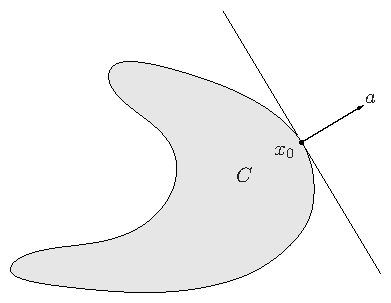
\includegraphics[width=.65\textwidth]{figures/ch02-figure-21.pdf}
\caption*{图2.21\quad 超平面 $\{x\mid a^{\T}x=a^{\T}x_0\}$ 在 $x_0$ 处支撑 $C$。}
\end{figure}
一个称为\emph{支撑超平面定理}的基本结果指出：对任意非空凸集 $C$ 和任意 $x_0\in\operatorname{bd}C$，都存在 $C$ 在 $x_0$ 处的支撑超平面。由分离超平面定理容易证明这一结果，分两种情形。若 $C$ 的内部非空，则对 $\{x_0\}$ 和 $\operatorname{int}C$ 应用分离超平面定理即可。若 $C$ 的内部为空，则 $C$ 必位于维数小于 $n$ 的仿射集中，任何包含这一仿射集的超平面都包含 $C$ 和 $x_0$，因此是一个平凡的支撑超平面。

支撑超平面定理也有部分逆命题：如果集合闭、内部非空，且每个边界点处都有支撑超平面，那么该集合凸，见习题2.27。

\section{对偶锥与广义不等式}
\subsection{对偶锥}
设 $K$ 是一个锥，集合
\begin{equation}
 K^*=\{y\mid x^{\T}y\ge0,\ \text{对所有 }x\in K\}\tag{2.19}
\end{equation}
称为 $K$ 的\emph{对偶锥}。顾名思义，$K^*$ 是一个锥，而且它总是凸的，即使原来的锥 $K$ 非凸也如此，见习题2.31。

几何上，$y\in K^*$ 当且仅当 $-y$ 是一个在原点支撑 $K$ 的超平面的法向量，见图2.22。

\begin{origexample}{2.22}
\textbf{子空间。}子空间 $V\subseteq\R^n$ 也是一个锥，其对偶锥为正交补
\[
 V^{\perp}=\{y\mid v^{\T}y=0,\ \text{对所有 }v\in V\}.
\]
\end{origexample}

% Source PDF page 66 (printed p. 52)
\begin{figure}[htbp]\centering
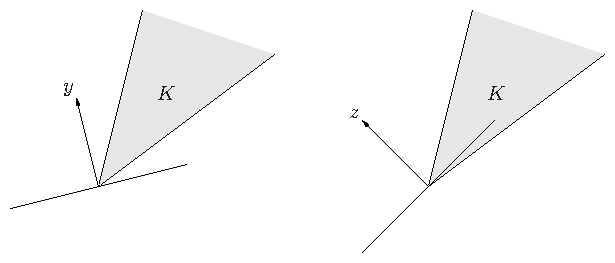
\includegraphics[width=.80\textwidth]{figures/ch02-figure-22.pdf}
\caption*{图2.22\quad 左：内法向量为 $y$ 的半空间包含锥 $K$，因此 $y\in K^*$。右：内法向量为 $z$ 的半空间不包含 $K$，因此 $z\notin K^*$。}
\end{figure}

\begin{origexample}{2.23}
\textbf{非负正交锥。}锥 $\R_+^n$ 的对偶是自身：
\[
 x^{\T}y\ge0\ \text{对所有 }x\succeq0
 \quad\Longleftrightarrow\quad y\succeq0.
\]
这样的锥称为\emph{自对偶锥}。
\end{origexample}

\begin{origexample}{2.24}
\textbf{半正定锥。}在对称 $n\times n$ 矩阵空间 $\mathbf S^n$ 上，采用标准内积
$\tr(XY)=\sum_{i,j=1}^nX_{ij}Y_{ij}$，见第A.1.1节。半正定锥 $\mathbf S_+^n$ 自对偶，即对 $X,Y\in\mathbf S^n$，有
\[
 \tr(XY)\ge0\ \text{对所有 }X\succeq0
 \quad\Longleftrightarrow\quad Y\succeq0.
\]
下面证明这一点。

若 $Y\notin\mathbf S_+^n$，则存在 $q\in\R^n$，使
\[
 q^{\T}Yq=\tr(qq^{\T}Y)<0.
\]
于是，半正定矩阵 $X=qq^{\T}$ 满足 $\tr(XY)<0$，从而 $Y\notin(\mathbf S_+^n)^*$。

再设 $X,Y\in\mathbf S_+^n$。由特征值分解可写 $X=\sum_{i=1}^n\lambda_iq_iq_i^{\T}$，其中各特征值 $\lambda_i\ge0$，$i=1,\ldots,n$。因此
\[
 \tr(YX)=\tr\left(Y\sum_{i=1}^n\lambda_iq_iq_i^{\T}\right)
 =\sum_{i=1}^n\lambda_iq_i^{\T}Yq_i\ge0,
\]
故 $Y\in(\mathbf S_+^n)^*$。
\end{origexample}

\begin{origexample}{2.25}
\textbf{范数锥的对偶。}设 $\norm{\cdot}$ 是 $\R^n$ 上的范数。相关锥
$K=\{(x,t)\in\R^{n+1}\mid\norm x\le t\}$ 的对偶，是由对偶范数定义的锥，即
\[
 K^*=\{(u,v)\in\R^{n+1}\mid\norm u_*\le v\},
\]
其中对偶范数为 $\norm u_*=\sup\{u^{\T}x\mid\norm x\le1\}$，见（A.1.6）。

% Source PDF page 67 (printed p. 53)
要证明这一结果，需说明
\begin{equation}
 \bigl[x^{\T}u+tv\ge0\ \text{只要 }\norm x\le t\bigr]
 \quad\Longleftrightarrow\quad\norm u_*\le v.\tag{2.20}
\end{equation}
先证明关于 $(u,v)$ 的右侧条件蕴含左侧条件。设 $\norm u_*\le v$，且对某个 $t>0$ 有 $\norm x\le t$。如果 $t=0$，则 $x$ 必为零，显然 $u^{\T}x+vt\ge0$。由对偶范数定义及 $\norm{-x/t}\le1$，有
\[
 u^{\T}(-x/t)\le\norm u_*\le v,
\]
因而 $u^{\T}x+vt\ge0$。

再证明（2.20）左侧蕴含右侧。假设 $\norm u_*>v$，即右侧不成立。由对偶范数定义，存在 $x$，满足 $\norm x\le1$ 且 $x^{\T}u>v$。取 $t=1$，有
\[
 u^{\T}(-x)+v<0,
\]
与（2.20）左侧条件矛盾。
\end{origexample}

对偶锥满足以下性质：
\begin{itemize}
\item $K^*$ 闭且凸。
\item $K_1\subseteq K_2$ 蕴含 $K_2^*\subseteq K_1^*$。
\item 如果 $K$ 的内部非空，则 $K^*$ 尖。
\item 如果 $K$ 的闭包尖，则 $K^*$ 内部非空。
\item $K^{**}$ 是 $K$ 的凸包的闭包。因此，若 $K$ 凸且闭，则 $K^{**}=K$。
\end{itemize}
见习题2.31。这些性质表明，如果 $K$ 是正常锥，则对偶锥 $K^*$ 也正常，而且 $K^{**}=K$。

\subsection{对偶广义不等式}
现在，设凸锥 $K$ 正常，从而诱导广义不等式 $\preceq_K$。对偶锥 $K^*$ 也正常，因此同样诱导一个广义不等式。将 $\preceq_{K^*}$ 称为 $\preceq_K$ 的\emph{对偶广义不等式}。两者的重要联系包括：
\begin{itemize}
\item $x\preceq_K y$，当且仅当对所有 $\lambda\succeq_{K^*}0$，有 $\lambda^{\T}x\le\lambda^{\T}y$。
\item $x\prec_K y$，当且仅当对所有 $\lambda\succeq_{K^*}0$、$\lambda\ne0$，有 $\lambda^{\T}x<\lambda^{\T}y$。
\end{itemize}
由于 $K=K^{**}$，$\preceq_{K^*}$ 的对偶广义不等式是 $\preceq_K$，所以上述性质在交换广义不等式与其对偶后仍成立。例如，$\lambda\preceq_{K^*}\mu$，当且仅当对所有 $x\succeq_K0$，有 $\lambda^{\T}x\le\mu^{\T}x$。

% Source PDF page 68 (printed p. 54)
\begin{origexample}{2.26}
\textbf{严格线性广义不等式的择一定理。}设 $K\subseteq\R^m$ 为正常锥，考虑严格广义不等式
\begin{equation}
 Ax\prec_K b,\tag{2.21}
\end{equation}
其中 $x\in\R^n$。

我们推导这一不等式的择一定理。假设它不可行，即仿射集 $\{b-Ax\mid x\in\R^n\}$ 与开凸集 $\operatorname{int}K$ 不相交。那么存在分离超平面，即非零 $\lambda\in\R^m$ 和 $\mu\in\R$，使对所有 $x$ 有 $\lambda^{\T}(b-Ax)\le\mu$，对所有 $y\in\operatorname{int}K$ 有 $\lambda^{\T}y\ge\mu$。第一个条件推出 $A^{\T}\lambda=0$、$\lambda^{\T}b\le\mu$。第二个条件推出对所有 $y\in K$ 有 $\lambda^{\T}y\ge\mu$，这只有在 $\lambda\in K^*$ 且 $\mu\le0$ 时才可能成立。

综合可得，如果（2.21）不可行，则存在 $\lambda$ 满足
\begin{equation}
 \lambda\ne0,\qquad\lambda\succeq_{K^*}0,\qquad
 A^{\T}\lambda=0,\qquad\lambda^{\T}b\le0.\tag{2.22}
\end{equation}
再证明逆命题：若（2.22）成立，则不等式组（2.21）必不可行。假设两者都成立。由于 $\lambda\ne0$、$\lambda\succeq_{K^*}0$、$b-Ax\succ_K0$，有 $\lambda^{\T}(b-Ax)>0$。但由 $A^{\T}\lambda=0$ 又得 $\lambda^{\T}(b-Ax)=\lambda^{\T}b\le0$，矛盾。

因此，不等式组（2.21）与（2.22）互为择一系统：对任意 $A,b$，恰有一个可行。这推广了 $K=\R_+^m$ 时的择一系统（2.17）、（2.18）。
\end{origexample}

\subsection{通过对偶不等式刻画最小元与极小元}
可用对偶广义不等式刻画集合 $S\subseteq\R^m$ 关于正常锥 $K$ 所诱导广义不等式的最小元与极小元，这里的 $S$ 可以非凸。

\subsubsection*{最小元的对偶刻画}
先考虑最小元的刻画：$x$ 是 $S$ 关于 $\preceq_K$ 的最小元，当且仅当对所有 $\lambda\succ_{K^*}0$，$x$ 都是在 $z\in S$ 上最小化 $\lambda^{\T}z$ 的唯一解。几何上，这意味着对任意 $\lambda\succ_{K^*}0$，超平面
\[
 \{z\mid\lambda^{\T}(z-x)=0\}
\]
都是 $S$ 在 $x$ 处的严格支撑超平面。“严格支撑”指超平面与 $S$ 仅在 $x$ 处相交。这里不要求 $S$ 凸，见图2.23。

为证明这一结果，假设 $x$ 是 $S$ 的最小元，即对所有 $z\in S$ 都有 $x\preceq_K z$，并取 $\lambda\succ_{K^*}0$。对 $z\in S$、$z\ne x$，由于 $x$ 是最小元，有 $z-x\succeq_K0$。结合 $\lambda\succ_{K^*}0$ 和 $z-x\ne0$，得 $\lambda^{\T}(z-x)>0$。$z$ 是 $S$ 中任意不同于 $x$ 的点，因此 $x$ 是 $\lambda^{\T}z$ 在 $S$ 上的唯一最小点。

反过来，假设对所有 $\lambda\succ_{K^*}0$，$x$ 都是 $\lambda^{\T}z$ 在 $S$ 上的唯一最小点，但 $x$ 不是 $S$ 的最小元。

% Source PDF page 69 (printed p. 55)
\begin{figure}[htbp]\centering
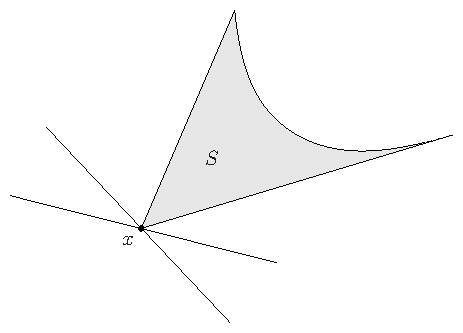
\includegraphics[width=.60\textwidth]{figures/ch02-figure-23.pdf}
\caption*{图2.23\quad 最小元的对偶刻画。$x$ 是集合 $S$ 关于 $\R_+^2$ 的最小元，等价地，对每个 $\lambda\succ0$，超平面 $\{z\mid\lambda^{\T}(z-x)=0\}$ 都在 $x$ 处严格支撑 $S$，即 $S$ 全部位于其一侧，且仅在 $x$ 处接触超平面。}
\end{figure}
那么存在 $z\in S$，使 $z\not\succeq_K x$。由于 $z-x\not\succeq_K0$，存在 $\widetilde\lambda\succeq_{K^*}0$，使 $\widetilde\lambda^{\T}(z-x)<0$。因此，在 $\widetilde\lambda$ 邻域内可取 $\lambda\succ_{K^*}0$，使 $\lambda^{\T}(z-x)<0$，这与 $x$ 是 $\lambda^{\T}z$ 在 $S$ 上的唯一最小点相矛盾。

\subsubsection*{极小元的对偶刻画}
接下来考虑极小元的类似刻画。这里的必要条件与充分条件之间存在差距。如果 $\lambda\succ_{K^*}0$，且 $x$ 在 $z\in S$ 上最小化 $\lambda^{\T}z$，则 $x$ 是极小元，见图2.24。

为证明这一点，设 $\lambda\succ_{K^*}0$，且 $x$ 在 $S$ 上最小化 $\lambda^{\T}z$，但 $x$ 不是极小元。也就是说，存在 $z\in S$、$z\ne x$ 且 $z\preceq_K x$。于是 $\lambda^{\T}(x-z)>0$，与 $x$ 是 $S$ 上的最小点这一假设矛盾。

逆命题一般不成立：某点 $x$ 可以是 $S$ 的极小元，却对任意 $\lambda$ 都不是 $\lambda^{\T}z$ 在 $S$ 上的最小点，见图2.25。这个图提示凸性在逆命题中起着重要作用，事实也确实如此。若 $S$ 凸，则对每个极小元 $x$，都存在非零 $\lambda\succeq_{K^*}0$，使 $x$ 在 $S$ 上最小化 $\lambda^{\T}z$。

为证明这一点，设 $x$ 极小，即 $((x-K)\setminus\{x\})\cap S=\varnothing$。对凸集 $(x-K)\setminus\{x\}$ 和 $S$ 应用分离超平面定理，得存在 $\lambda\ne0$ 和 $\mu$，使对所有 $y\in K$ 有 $\lambda^{\T}(x-y)\le\mu$，对所有 $z\in S$ 有 $\lambda^{\T}z\ge\mu$。第一个不等式推出 $\lambda\succeq_{K^*}0$。因为 $x\in S$ 且 $x\in x-K$，有 $\lambda^{\T}x=\mu$，第二个不等式因此表明，$\mu$ 是 $\lambda^{\T}z$ 在 $S$ 上的最小值。所以，$x$ 是 $\lambda^{\T}z$ 在 $S$ 上的最小点，其中 $\lambda\ne0$、$\lambda\succeq_{K^*}0$。

这个逆定理中的条件不能加强为 $\lambda\succ_{K^*}0$。例子表明，一个点 $x$ 可以是凸集 $S$ 的极小点，却对任意 $\lambda\succ_{K^*}0$ 都不是 $\lambda^{\T}z$ 在 $S$ 上的最小点。

% Source PDF page 70 (printed p. 56)
\begin{figure}[htbp]\centering
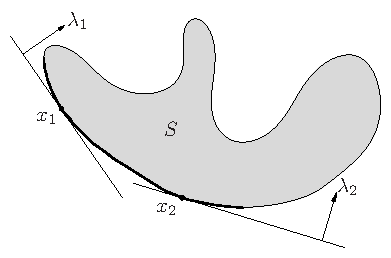
\includegraphics[width=.66\textwidth]{figures/ch02-figure-24.pdf}
\caption*{图2.24\quad 集合 $S\subseteq\R^2$。关于 $\R_+^2$ 的极小点集，是左下边界上以深色表示的部分。$\lambda_1^{\T}z$ 在 $S$ 上的最小点为 $x_1$，由于 $\lambda_1\succ0$，它是极小点。$\lambda_2^{\T}z$ 在 $S$ 上的最小点为 $x_2$，由于 $\lambda_2\succ0$，它也是 $S$ 的极小点。}
\end{figure}
\begin{figure}[htbp]\centering
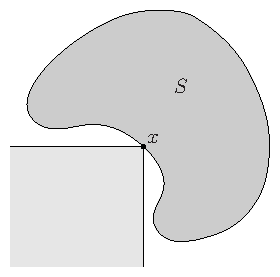
\includegraphics[width=.60\textwidth]{figures/ch02-figure-25.pdf}
\caption*{图2.25\quad 点 $x$ 是 $S\subseteq\R^2$ 关于 $\R_+^2$ 的极小元，但不存在使 $x$ 在 $z\in S$ 上最小化 $\lambda^{\T}z$ 的 $\lambda$。}
\end{figure}

% Source PDF page 71 (printed p. 57)
\begin{figure}[htbp]\centering
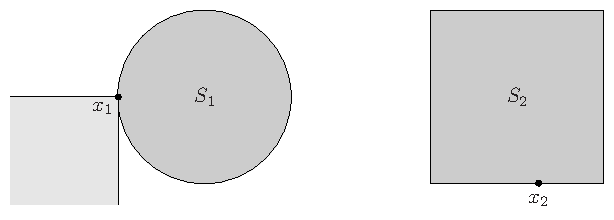
\includegraphics[width=.82\textwidth]{figures/ch02-figure-26.pdf}
\caption*{图2.26\quad 左：点 $x_1\in S_1$ 极小，但对任意 $\lambda\succ0$，都不是 $\lambda^{\T}z$ 在 $S_1$ 上的最小点。不过，当 $\lambda=(1,0)$ 时，它确实在 $z\in S_1$ 上最小化 $\lambda^{\T}z$。右：点 $x_2\in S_2$ 不极小，但当 $\lambda=(0,1)\succeq0$ 时，它是在 $z\in S_2$ 上最小化 $\lambda^{\T}z$ 的点。}
\end{figure}
前述不能加强条件的情形见图2.26左图。同时，也不能说：当 $\lambda\succeq_{K^*}0$ 时，$\lambda^{\T}z$ 在 $S$ 上的每个最小点都是极小元，见图2.26右图。

\begin{origexample}{2.27}
\textbf{Pareto最优生产前沿。}考虑制造某种产品，需要使用 $n$ 种资源，例如劳动力、电力、天然气和水。产品有多种制造或生产方法。对每种生产方法，关联资源向量 $x\in\R^n$，$x_i$ 表示该方法生产产品所消耗的第 $i$ 种资源的数量。假设 $x_i\ge0$，即生产方法消耗资源；同时资源具有价值，因此任何一种资源都希望用得更少。

\emph{生产集} $P\subseteq\R^n$ 定义为所有对应某种生产方法的资源向量 $x$ 构成的集合。

若某种生产方法的资源向量是 $P$ 关于逐分量不等式的极小元，就称该生产方法为\emph{Pareto最优}或\emph{有效}的。$P$ 的极小元集称为\emph{有效生产前沿}。

Pareto最优性有一个简单解释。若资源向量为 $x$ 的方法与资源向量为 $y$ 的方法相比，满足所有 $i$ 都有 $x_i\le y_i$，并且至少一个 $i$ 有 $x_i<y_i$，就称前者\emph{优于}后者。换言之，一种方法在每项资源的使用量上都不超过另一种，并至少有一项严格更少，就更好。这对应 $x\preceq y$、$x\ne y$。因此可以说：没有更好的生产方法时，该生产方法就是Pareto最优或有效的。

选择任意满足 $\lambda\succ0$ 的 $\lambda$，在生产向量集 $P$ 上最小化
\[
 \lambda^{\T}x=\lambda_1x_1+\cdots+\lambda_nx_n,
\]
便能找到Pareto最优生产方法，即极小资源向量。

向量 $\lambda$ 有简单的解释：$\lambda_i$ 是第 $i$ 种资源的价格。在 $P$ 上最小化 $\lambda^{\T}x$，就是寻找给定资源价格 $\lambda_i$ 下总成本最低的生产方法。只要价格均为正，得到的生产方法就保证有效。

图2.27说明了这些概念。
\end{origexample}

% Source PDF page 72 (printed p. 58)
\begin{figure}[htbp]\centering
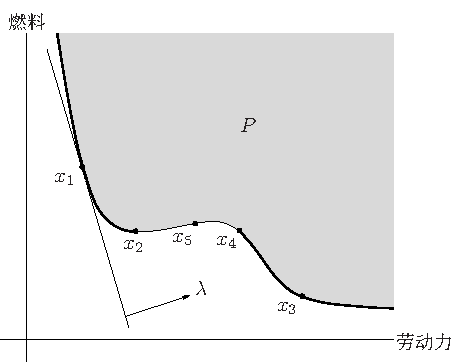
\includegraphics[width=.70\textwidth]{figures/ch02-figure-27.pdf}
\caption*{图2.27\quad 生产某种产品所需的资源为劳动力与燃料，生产集 $P$ 以阴影表示。两条深色曲线是有效生产前沿。点 $x_1$、$x_2$、$x_3$ 有效；点 $x_4$ 和 $x_5$ 无效，特别地，$x_2$ 对应的方法燃料用量不更多，劳动力用量更少。$x_1$ 还是正价格向量 $\lambda$ 下成本最低的生产方法。$x_2$ 有效，但不能通过对任何价格向量 $\lambda\succeq0$ 最小化总成本 $\lambda^{\T}x$ 找到。}
\end{figure}
